\documentclass[12pt]{extarticle}
\usepackage[english]{babel}
\usepackage[utf8]{inputenc}
\usepackage[english]{babel}
\usepackage[a4paper, total={7.25in, 9.5in}]{geometry}
\usepackage{tikz-feynman}
\tikzfeynmanset{compat=1.0.0} 
\usepackage{subcaption}
\usepackage{float}
\floatplacement{figure}{H}
\usepackage{simpler-wick}
\usepackage{mathrsfs}  
\usepackage{dsfont}
\usepackage{relsize}
\usepackage{tikz-cd}
\DeclareMathAlphabet{\mathdutchcal}{U}{dutchcal}{m}{n}

\usepackage{cancel}



\newcommand{\field}{\hat{\Phi}}
\newcommand{\dfield}{\hat{\Phi}^\dagger}
 
\usepackage{amsthm, amssymb, amsmath, centernot}
\usepackage{slashed}
\newcommand{\notimplies}{%
  \mathrel{{\ooalign{\hidewidth$\not\phantom{=}$\hidewidth\cr$\implies$}}}}
 
\renewcommand\qedsymbol{$\square$}
\newcommand{\cont}{$\boxtimes$}
\newcommand{\divides}{\mid}
\newcommand{\ndivides}{\centernot \mid}

\newcommand{\Integers}{\mathbb{Z}}
\newcommand{\Natural}{\mathbb{N}}
\newcommand{\Complex}{\mathbb{C}}
\newcommand{\Zplus}{\mathbb{Z}^{+}}
\newcommand{\Primes}{\mathbb{P}}
\newcommand{\Q}{\mathbb{Q}}
\newcommand{\R}{\mathbb{R}}
\newcommand{\ball}[2]{B_{#1} \! \left(#2 \right)}
\newcommand{\Rplus}{\mathbb{R}^+}
\renewcommand{\Re}[1]{\mathrm{Re}\left[ #1 \right]}
\renewcommand{\Im}[1]{\mathrm{Im}\left[ #1 \right]}
\newcommand{\Op}{\mathcal{O}}

\newcommand{\invI}[2]{#1^{-1} \left( #2 \right)}
\newcommand{\End}[1]{\text{End}\left( A \right)}
\newcommand{\legsym}[2]{\left(\frac{#1}{#2} \right)}
\renewcommand{\mod}[3]{\: #1 \equiv #2 \: \mathrm{mod} \: #3 \:}
\newcommand{\nmod}[3]{\: #1 \centernot \equiv #2 \: mod \: #3 \:}
\newcommand{\ndiv}{\hspace{-4pt}\not \divides \hspace{2pt}}
\newcommand{\finfield}[1]{\mathbb{F}_{#1}}
\newcommand{\finunits}[1]{\mathbb{F}_{#1}^{\times}}
\newcommand{\ord}[1]{\mathrm{ord}\! \left(#1 \right)}
\newcommand{\quadfield}[1]{\Q \small(\sqrt{#1} \small)}
\newcommand{\vspan}[1]{\mathrm{span}\! \left\{#1 \right\}}
\newcommand{\galgroup}[1]{Gal \small(#1 \small)}
\newcommand{\bra}[1]{\left| #1 \right>}
\newcommand{\Oa}{O_\alpha}
\newcommand{\Od}{O_\alpha^{\dagger}}
\newcommand{\Oap}{O_{\alpha '}}
\newcommand{\Odp}{O_{\alpha '}^{\dagger}}
\newcommand{\im}[1]{\mathrm{im} \: #1}
\renewcommand{\ker}[1]{\mathrm{ker} \: #1}
\newcommand{\ket}[1]{\left| #1 \right>}
\renewcommand{\bra}[1]{\left< #1 \right|}
\newcommand{\inner}[2]{\left< #1 | #2 \right>}
\newcommand{\expect}[2]{\left< #1 \right| #2 \left| #1 \right>}
\renewcommand{\d}[1]{ \mathrm{d}#1 \:}
\newcommand{\dn}[2]{ \mathrm{d}^{#1} #2 \:}
\newcommand{\deriv}[2]{\frac{\d{#1}}{\d{#2}}}
\newcommand{\nderiv}[3]{\frac{\dn{#1}{#2}}{\d{#3^{#1}}}}
\newcommand{\pderiv}[2]{\frac{\partial{#1}}{\partial{#2}}}
\newcommand{\fderiv}[2]{\frac{\delta #1}{\delta #2}}
\newcommand{\parsq}[2]{\frac{\partial^2{#1}}{\partial{#2}^2}}
\newcommand{\topo}{\mathcal{T}}
\newcommand{\base}{\mathcal{B}}
\renewcommand{\bf}[1]{\mathbf{#1}}
\renewcommand{\a}{\hat{a}}
\newcommand{\adag}{\hat{a}^\dagger}
\renewcommand{\b}{\hat{b}}
\newcommand{\bdag}{\hat{b}^\dagger}
\renewcommand{\c}{\hat{c}}
\newcommand{\cdag}{\hat{c}^\dagger}
\newcommand{\hamilt}{\hat{H}}
\renewcommand{\L}{\hat{L}}
\newcommand{\Lz}{\hat{L}_z}
\newcommand{\Lsquared}{\hat{L}^2}
\renewcommand{\S}{\hat{S}}
\renewcommand{\empty}{\varnothing}
\newcommand{\J}{\hat{J}}
\newcommand{\lagrange}{\mathcal{L}}
\newcommand{\dfourx}{\mathrm{d}^4x}
\newcommand{\meson}{\phi}
\newcommand{\dpsi}{\psi^\dagger}
\newcommand{\ipic}{\mathrm{int}}
\newcommand{\tr}[1]{\mathrm{tr} \left( #1 \right)}
\newcommand{\C}{\mathbb{C}}
\newcommand{\CP}[1]{\mathbb{CP}^{#1}}
\newcommand{\Vol}[1]{\mathrm{Vol}\left(#1\right)}

\newcommand{\Tr}[1]{\mathrm{Tr}\left( #1 \right)}
\newcommand{\Charge}{\hat{\mathbf{C}}}
\newcommand{\Parity}{\hat{\mathbf{P}}}
\newcommand{\Time}{\hat{\mathbf{T}}}
\newcommand{\Torder}[1]{\mathbf{T}\left[ #1 \right]}
\newcommand{\Norder}[1]{\mathbf{N}\left[ #1 \right]}
\newcommand{\Znorm}{\mathcal{Z}}
\newcommand{\EV}[1]{\left< #1 \right>}
\newcommand{\interact}{\mathrm{int}}
\newcommand{\covD}{\mathcal{D}}
\newcommand{\conj}[1]{\overline{#1}}

\newcommand{\SO}[2]{\mathrm{SO}(#1, #2)}
\newcommand{\SU}[2]{\mathrm{SU}(#1, #2)}

\newcommand{\anticom}[2]{\left\{ #1 , #2 \right\}}


\newcommand{\pathd}[1]{\! \mathdutchcal{D} #1 \:}

\renewcommand{\theenumi}{(\alph{enumi})}


\renewcommand{\theenumi}{(\alph{enumi})}

\newcommand{\atitle}[1]{\title{% 
	\large \textbf{Physics GR8048 Quantum Field Theory II
	\\ Assignment \# #1} \vspace{-2ex}}
\author{Benjamin Church }
\maketitle}

\newcommand{\atitleIII}[1]{\title{% 
	\large \textbf{Physics GR8049 Quantum Field Theory III
	\\ Assignment \# #1} \vspace{-2ex}}
\author{Benjamin Church }
\maketitle}

\theoremstyle{definition}
\newtheorem{theorem}{Theorem}[section]
\newtheorem{definition}{definition}[section]
\newtheorem{lemma}[theorem]{Lemma}
\newtheorem{proposition}[theorem]{Proposition}
\newtheorem{corollary}[theorem]{Corollary}
\newtheorem{example}[theorem]{Example}
\newtheorem{remark}[theorem]{Remark}


\begin{document}
\atitle{3}
 
\section*{Problem 1.}
To save space, I will write, $\phi_i = \phi(x_i)$ and $\Delta_{ij} = \Delta(x_i - x_j)$. First, we will flesh out the inductive proof of Wick's theorem. Assuming the inductive hypothesis, that Wick's theorem holds for $3$ fields. Now, consider the time ordered product of $4$ fields,
	\[ \mathbf{T} \phi(x_1) \phi(x_2) \phi(x_3) \phi(x_4)\]
Without loss of generality, assume that $x_1^0 > x_i^0$ for $i = 1,2,3$. If this is not the case, the time-ordered product can be rearanged into the desired form by relabeling points. Furthermore we may decompose $\phi_1 = \phi_1^+ + \phi_1^-$, where $\phi_1^-$ contains only creation operators and $\phi_1^+$ contains only annihilation operators. Therefore,
	\[ \mathbf{T} \phi_1\phi_2\phi_3\phi_4 = \phi_1 \mathbf{T}\phi_2\phi_3\phi_4 = (\phi_1^+ + \phi_1^-) \left(
	: \phi_2 \phi_3 \phi_4 : + \phi_2 \Delta_{34} + \phi_3 \Delta_{24} + \phi_4 \Delta_{23} \right) \]
To normal order this expression, we need to move $\phi_1^+$ to the right of the other field operators. However, using the fact that $x_1^0 > x_2^0$, we have, $[\phi_1^+, \phi_2] = [\phi_1^+, \phi_2^+ + \phi_2^-] = [\phi_1^+, \phi_2^-] = \Delta_{12}$ since $[\phi_1^+, \phi_2^+]$ commute with eachother due to the fact that all annihlation operators commute. Therefore,
\[ \phi_1 \phi_2 = \: : \phi_1 \phi_2 : + \Delta_{12} \] 
and a similar relation holds for any other of the contractions. Thus, 
\[ \mathbf{T} \phi_1\phi_2\phi_3\phi_4 = (\phi_1^+ + \phi_1^-) : \phi_2 \phi_3 \phi_4 : + :\phi_1 \phi_2: \Delta_{34} + \Delta_{12} \Delta_{34} + :\phi_1 \phi_3 : \Delta_{24} + \Delta_{13} \Delta_{24} + : \phi_1  \phi_4: \Delta_{23} + \Delta_{14} \Delta_{23} \]
Now we must deal with the first term,	
	
\begin{align*} 
(\phi_1^+ + \phi_1^-) : \phi_2 \phi_3 \phi_4 : & = \phi_1^- : \phi_2 \phi_3 \phi_4 : + [\phi_1^+, \phi_2] : \phi_3 \phi_4 : + \phi_2 \phi_1^+ : \phi_3 \phi_4 : 
\\
& = \phi_1^- : \phi_2 \phi_3 \phi_4 : +  : \phi_3 \phi_4 : \Delta_{12} + :\phi_2 [\phi_1^+ , \phi_3] \phi_4 : + :\phi_2 \phi_3 \phi_1^+ \phi_4 : 
\\
& = \phi_1^- : \phi_2 \phi_3 \phi_4 : + : \phi_3 \phi_4 : \Delta_{12} + :\phi_2 \phi_4 : \Delta_{13} + :\phi_2 \phi_3 [\phi_1^+, \phi_4] : + : \phi_2 \phi_2 \phi_3 : \phi_1^+
\\
& = : \phi_1 \phi_2 \phi_3 \phi_4: + : \phi_3 \phi_4 : \Delta_{12} + :\phi_2 \phi_4 : \Delta_{13} + :\phi_2 \phi_3 : \Delta_{14}
\end{align*}
Putting everything together,
\begin{align*}
\mathbf{T} \phi_1\phi_2\phi_3\phi_4  =  \: \: & : \phi_1 \phi_2 \phi_3 \phi_4: +  \Delta_{12} : \phi_3 \phi_4 : + \Delta_{13} :\phi_2 \phi_4 : + \Delta_{14} : \phi_2 \phi_3 : + \Delta_{23} : \phi_1  \phi_4: + \Delta_{24} :\phi_1 \phi_3 :
\\ 
& + \Delta_{34} : \phi_1 \phi_2 : + \Delta_{12} \Delta_{34} + \Delta_{13} \Delta_{24}  + \Delta_{14} \Delta_{23}
\end{align*}
\section*{Problem 2.}
Write the Lagrangian,
\[ \lagrange = \lagrange_0 + \lagrange_{\ipic} \quad \quad \lagrange_0 = \tfrac{1}{2} \partial_\mu \phi \partial^\mu \phi - \tfrac{1}{2} m^2 \phi^2 + \partial_\mu \dpsi \partial^\mu \psi - M^2 \dpsi \psi \quad \quad \lagrange_{\ipic} = -g \dpsi \psi \meson \] 
\subsection*{(a)}
For nucleon-antinucleon scattering, using relativistic normalization, the initial and final states are: 
\[\ket{i} = \sqrt{2 E_1} \sqrt{2 E_2} \bdag_{\vec{p}_1} \cdag_{\vec{p}_2} \ket{0}\quad \quad \ket{f} = \sqrt{2 E_1'} \sqrt{2 E_2'} \bdag_{\vec{p'}_1} \cdag_{\vec{p'}_2} \ket{0} \]
Expanding the Dyson series to second order,
\[ A = \bra{f} \left( \mathbf{1} + (- ig) \int \dfourx \: \dpsi(x) \psi(x) \meson(x) +  (- ig)^2 \frac{1}{2} \int\int \dfourx_1 \dfourx_2 \mathrm{T} \: \dpsi(x_1) \psi(x_1) \meson(x_1) \dpsi(x_2) \psi(x_2) \meson(x_2)  \right) \ket{i} \]
We can ignore the first and second term in this expansion. The first term is a delta-function representing the case of no interaction. The second term is identically zero because there is a lonly $\phi$ which cannot contract with anything. Fousing on the third term,
\begin{align*}
& = (- ig)^2 \frac{1}{2} \int\int \dfourx_1 \dfourx_2 \: \bra{f} \mathrm{T} \: \dpsi(x_1) \psi(x_1) \meson(x_1) \dpsi(x_2) \psi(x_2) \meson(x_2) \ket{i} \\
\end{align*}
Using Wick's theorem, we can rewrite the inner product in terms of normal ordered operators. Considering only connected diagrams (i.e. no contraction of creation/ahiliation operations in the initial state with those in the final state which require independent conservation of momentum of the individual particles), there is only one term in the Wick expansion which does not give zero. This term comes from the contraction of the meson fields,
\[ \Delta_F^{(\phi)}(x_1 - x_2)\: :\dpsi(x_1) \psi(x_1) \dpsi(x_2) \psi(x_2):\] 
No other terms can contribute because they would either have uncontracted meson fields which anhilate the initial and final states or not enough uncontracted field operators to operate on each of the four incoming/outgoing particle states. Therefore,
\begin{align*}
A & = (- ig)^2 \frac{1}{2} \int\int \dfourx_1 \dfourx_2 \: \Delta_F^{(\phi)}(x_1 - x_2) \bra{p'_1 p'_2} : \dpsi(x_1) \psi(x_1) \dpsi(x_2) \psi(x_2) :\ket{p_1 p_2}
\\
& = (- ig)^2 \frac{1}{2} \int\int \dfourx_1 \dfourx_2 \: \Delta_F^{(\phi)}(x_1 - x_2) \left(e^{- i p_1 x_1} e^{i p_2' x_2} + e^{- i p_1 x_2 } e^{i p_2' x_1} \right) \left( e^{- i p_2 x_1} e^{i p_1' x_2} + e^{- i p_2 x_2} e^{i p_1' x_1}  \right)
\\
& = (- ig)^2 \frac{1}{2} \int\int \dfourx_1 \dfourx_2 \: \int \d{k} \frac{i}{k^2 - m^2 + i \epsilon}  
\\
& \cdot \left( e^{-i (p_1 + p_2 + k) x_1} e^{i (p_2' + p_1' + k) x_2} + e^{i (p_1' - p_1 - k) x_1} e^{i (p_2' - p_2 + k) x_2} + e^{i (p_2' - p_2 - k) x_1} e^{i(p_1' - p_1 + k)x_2} + e^{i(p_1' + p_2' - k) x_1} e^{-i(p_1 + p_2 - k) x_2} \right)
\\
& = (- ig)^2 \frac{(2 \pi)^4}{2} \: \int \d{k} \frac{i}{k^2 - m^2 + i \epsilon}  \cdot \left( \delta^4(p_1 + p_2 + k) \delta^4(p_2' + p_1' + k) + \delta^4(p_1' - p_1 - k) \delta^4(p_2' - p_2 + k) \right. 
\\
& \quad \quad \left. + \delta^4(p_2' - p_2 - k) \delta^4(p_1' - p_1 + k) + \delta^4(p_1' + p_2' - k) \delta^4(p_1 + p_2 - k)  \right)
\\
& = (- ig)^2 (2 \pi)^4 \delta^4(p_1 + p_2 - p_1' - p_2') \left[ \frac{i}{(p_1 + p_2)^2 - m^2 + i \epsilon} + \frac{i}{(p_1 - p_1')^2 - m^2 + i \epsilon} \right]
\end{align*}

\subsection*{(b)}
At second order, there are two contributions to the nucleon-antinucleon scattering,
\begin{figure}
\centering
\begin{minipage}{.5\textwidth}
  \centering
  
\feynmandiagram [vertical=b to a] {
i1 -- [fermion, momentum = \(p_1\)] a -- [fermion, momentum = \(p_1'\)] f1,
a -- [scalar, edge label = \(\Delta_F\)] b,
f2 -- [fermion, momentum' = \(p_2\)] b -- [fermion, momentum' = \(p_2'\)] i2,
};

\end{minipage}%
\begin{minipage}{.5\textwidth}
  \centering
  
\feynmandiagram [horizontal=a to b] {
i1 -- [fermion, momentum = \(p_1\)] a -- [fermion, rmomentum = \(p_2\)] i2,
a -- [scalar, edge label = \(\Delta_F\)] b,
f1 -- [fermion, rmomentum' = \(p_1'\)] b -- [fermion, momentum' = \(p_2'\)] f2,
};

\end{minipage}
\end{figure}
Using the Feynman rules, the amplitude for this process is given by,
\[ A = (- i g)^2 (2 \pi)^4 \delta^4(p_1 + p_2 - p_1' - p_2') \left[ \frac{i}{(p_1 - p_1')^2 - m^2 + i \epsilon} + \frac{i}{(p_1 + p_2)^2 - m^2 + i \epsilon} \right] \]
where each vertex contributes a factor of $(-ig)$. 
\subsection*{(c)}
There are no terms at third order because every term would have an uncontracted $\phi$ term. At fourth order, the connected diagrams are,
\begin{center}
\feynmandiagram [baseline=(b.base), horizontal=b to d] {
a -- [fermion] b -- [fermion] c,
b -- [scalar] l1 
-- [fermion, half left, looseness=1.5] l2 
--[fermion, half left, looseness=1.5] l1,
l2 -- [scalar] d,
f2 -- [fermion] d -- [fermion] f1,
};
\end{center}
\begin{center}
\feynmandiagram [baseline=(b.base), horizontal=a to b] {
i1 -- [fermion] s1 -- [fermion] a,
a -- [fermion] s2 -- [fermion] i2,
f1 -- [fermion] b -- [fermion] f2,
s1 -- [scalar] s2,
a -- [scalar] b
};
\quad \quad
\feynmandiagram [baseline = (l2.base), vertical =b to d] {
a -- [fermion] b -- [fermion] c,
b -- [scalar] l1 
-- [fermion, half left, looseness=1.5] l2 
--[fermion, half left, looseness=1.5] l1,
l2 -- [scalar] d,
f2 -- [fermion] d -- [fermion] f1,
};
\quad \quad
\feynmandiagram [baseline=(b.base), horizontal=b to a] {
i1 -- [fermion] s1 -- [fermion] a,
a -- [fermion] s2 -- [fermion] i2,
f1 -- [fermion] b -- [fermion] f2,
s1 -- [scalar] s2,
a -- [scalar] b
};
\end{center}
\begin{center}
\feynmandiagram [horizontal=s1 to s2] {
i1 -- [fermion] s1 -- [fermion] s2 -- [fermion] f1,
f2 -- [fermion] s3 -- [fermion] s4 -- [fermion] i2,
s1 -- [scalar] s4,
s2 -- [scalar] s3
};
\quad \quad 
\feynmandiagram [horizontal=s1 to s4] {
i1 -- [fermion] s1 -- [fermion] s2 -- [fermion] i2,
f1 -- [fermion] s3 -- [fermion] s4 -- [fermion] f2,
s1 -- [scalar] s4,
s2 -- [scalar] s3
};
\quad \quad
\begin{tikzpicture}
\begin{feynman}
\vertex (i1) ;
\vertex [below right=of i1] (s1);
\vertex [right=of s1] (s2);
\vertex [below=of s2] (s3);
\vertex [left=of s3] (s4);
\vertex [below left=of s4] (i2);
\vertex [below right=of s3] (f2);
\vertex [above right=of s2] (f1);
\diagram* {
(i1) -- [fermion] (s1) -- [fermion] (s4) -- [fermion] (i2),
(f2) -- [fermion] (s3) -- [fermion] (s2) -- [fermion] (f1),
(s1) -- [scalar] (s3)
(s2) -- [scalar] (s4)
};
\end{feynman}
\end{tikzpicture}
\quad \quad
\begin{tikzpicture}
\begin{feynman}
\vertex (i1) ;
\vertex [below right=of i1] (s1);
\vertex [right=of s1] (s2);
\vertex [below=of s2] (s3);
\vertex [left=of s3] (s4);
\vertex [below left=of s4] (i2);
\vertex [below right=of s3] (f2);
\vertex [above right=of s2] (f1);
\diagram* {
(i1) -- [fermion] (s1) -- [fermion] (s2) -- [fermion] (f1),
(f2) -- [fermion] (s3) -- [fermion] (s4) -- [fermion] (i2),
(s1) -- [scalar] (s3)
(s2) -- [scalar] (s4)
};
\end{feynman}
\end{tikzpicture}
\end{center}

\begin{center}
	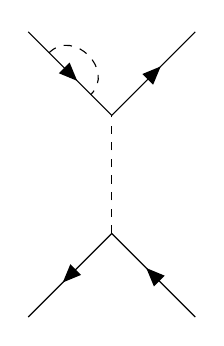
\begin{tikzpicture}
	\begin{feynman}
	\vertex (i1);
	\vertex[below right=of i1] (a);
	\vertex[above right=of a] (f1);
	\vertex[below=of a] (b);
	\vertex[below left=of b] (i2);
	\vertex[below right=of b] (f2);

	\vertex at ($(i1)!0.25!(a)$) (x);
	\vertex at ($(i1)!0.75!(a)$) (y);

	\diagram* {
	(i1) -- [fermion] (a) -- [fermion] (f1),
	(b) -- [scalar] (a),
	(f2) -- [fermion] (b) -- [fermion] (i2),
	(x) --[scalar, half left] (y)
	};
	\end{feynman}
	\end{tikzpicture}
	\hspace{1cm}
	\begin{tikzpicture}
	\begin{feynman}
	\vertex (i1);
	\vertex[below right=of i1] (a);
	\vertex[above right=of a] (f1);
	\vertex[below=of a] (b);
	\vertex[below left=of b] (i2);
	\vertex[below right=of b] (f2);

	\vertex at ($(i2)!0.25!(b)$) (x);
	\vertex at ($(i2)!0.75!(b)$) (y);

	\diagram* {
	(i1) -- [fermion] (a) -- [fermion] (f1),
	(b) -- [scalar] (a),
	(f2) -- [fermion] (b) -- [fermion] (i2)
	(x) --[scalar, half left] (y)
	};
	\end{feynman}
	\end{tikzpicture}
	\hspace{1cm}
	\begin{tikzpicture}
	\begin{feynman}
	\vertex (i1);
	\vertex[below right=of i1] (a);
	\vertex[above right=of a] (f1);
	\vertex[below=of a] (b);
	\vertex[below left=of b] (i2);
	\vertex[below right=of b] (f2);

	\vertex at ($(f1)!0.25!(a)$) (x);
	\vertex at ($(f1)!0.75!(a)$) (y);

	\diagram* {
	(i1) -- [fermion] (a) -- [fermion] (f1),
	(b) -- [scalar] (a),
	(f2) -- [fermion] (b) -- [fermion] (i2)
	(x) --[scalar, half right] (y)
	};
	\end{feynman}
	\end{tikzpicture}
	\hspace{1cm}
	\begin{tikzpicture}
	\begin{feynman}
	\vertex (i1);
	\vertex[below right=of i1] (a);
	\vertex[above right=of a] (f1);
	\vertex[below=of a] (b);
	\vertex[below left=of b] (i2);
	\vertex[below right=of b] (f2);

	\vertex at ($(f2)!0.25!(b)$) (x);
	\vertex at ($(f2)!0.75!(b)$) (y);

	\diagram* {
	(i1) -- [fermion] (a) -- [fermion] (f1),
	(b) -- [scalar] (a),
	(f2) -- [fermion] (b) -- [fermion] (i2)
	(x) --[scalar, half right] (y)
	};
	\end{feynman}
	\end{tikzpicture}
	\end{center}

\begin{center}
	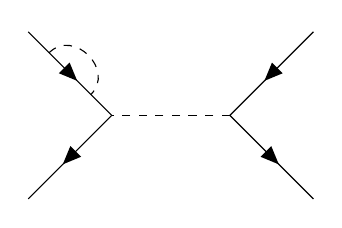
\begin{tikzpicture}
	\begin{feynman}
	\vertex (i1);
	\vertex[below right=of i1] (a);
	\vertex[right=of a] (b);
	\vertex[below left=of a] (i2);
	\vertex[above right=of b] (f1);
	\vertex[below right=of b] (f2);

	\vertex at ($(i1)!0.25!(a)$) (x);
	\vertex at ($(i1)!0.75!(a)$) (y);

	\diagram* {
	(i1) -- [fermion] (a) -- [fermion] (i2),
	(b) -- [scalar] (a),
	(f1) -- [fermion] (b) -- [fermion] (f2),
	(x) --[scalar, half left] (y)
	};
	\end{feynman}
	\end{tikzpicture}
	\hspace{2cm}
	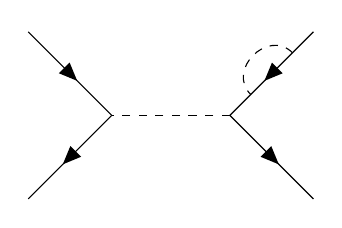
\begin{tikzpicture}
	\begin{feynman}
	\vertex (i1);
	\vertex[below right=of i1] (a);
	\vertex[right=of a] (b);
	\vertex[below left=of a] (i2);
	\vertex[above right=of b] (f1);
	\vertex[below right=of b] (f2);

	\vertex at ($(f1)!0.25!(b)$) (x);
	\vertex at ($(f1)!0.75!(b)$) (y);

	\diagram* {
	(i1) -- [fermion] (a) -- [fermion] (i2),
	(b) -- [scalar] (a),
	(f1) -- [fermion] (b) -- [fermion] (f2),
	(x) --[scalar, half right] (y)
	};
	\end{feynman}
	\end{tikzpicture}
	\end{center}
	\begin{center}
	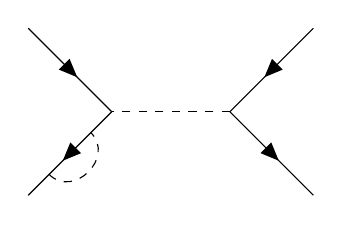
\begin{tikzpicture}
	\begin{feynman}
	\vertex (i1);
	\vertex[below right=of i1] (a);
	\vertex[right=of a] (b);
	\vertex[below left=of a] (i2);
	\vertex[above right=of b] (f1);
	\vertex[below right=of b] (f2);

	\vertex at ($(i2)!0.25!(a)$) (x);
	\vertex at ($(i2)!0.75!(a)$) (y);

	\diagram* {
	(i1) -- [fermion] (a) -- [fermion] (i2),
	(b) -- [scalar] (a),
	(f1) -- [fermion] (b) -- [fermion] (f2),
	(x) --[scalar, half right] (y)
	};
	\end{feynman}
	\end{tikzpicture}
	\hspace{2cm}
	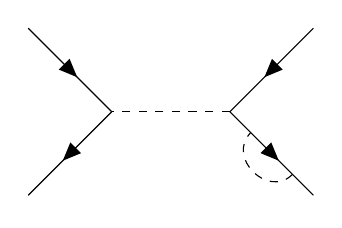
\begin{tikzpicture}
	\begin{feynman}
	\vertex (i1);
	\vertex[below right=of i1] (a);
	\vertex[right=of a] (b);
	\vertex[below left=of a] (i2);
	\vertex[above right=of b] (f1);
	\vertex[below right=of b] (f2);

	\vertex at ($(f2)!0.25!(b)$) (x);
	\vertex at ($(f2)!0.75!(b)$) (y);

	\diagram* {
	(i1) -- [fermion] (a) -- [fermion] (i2),
	(b) -- [scalar] (a),
	(f1) -- [fermion] (b) -- [fermion] (f2),
	(x) --[scalar, half left] (y)
	};
	\end{feynman}
	\end{tikzpicture}
	\end{center}		
Each of these terms has an unconstraned momentum which must be integrated over. In a simple two vertex loop, the unconstraned momentum will appear in exactly two propagators which gives a total order of $p^4$ the denominator. However, when integrated against $\mathrm{d}^4p$, this term diverges logarithmically. The square loops involving four propagators do not diverge but will generally be very difficult to calculate.    

\section*{Problem 3.}
Consider now the interation Lagrangian, 
\[ \lagrange_{\ipic} = - g \dpsi \psi \phi - \lambda (\dpsi \psi)^2\]
\subsection*{(a)}

The form of the vertex rules is clear from the terms which appear in the interaction Lagrangian. However, a combinatorial factor of $4$ appears in $(\psi^\dag \psi)^2$ vertices. To see this, consider the diagram resulting from a first order $\psi \overline{\psi} \to \psi \overline{\psi}$ process: 
	\begin{center}
	\feynmandiagram[small, vertical = i1 to i2] {
	i1 -- [fermion] a -- [fermion] i2,
	f1 -- [fermion] a -- [fermion] f2
	};
	\end{center}
Writing out the term in the Dyson expansion which leads to this diagram we have
	\[ (-i\lambda) \int \d{^4 x}
	\bra{p_1' p_2'}  : \psi^\dag(x) \psi^\dag(x) \psi(x) \psi(x) : \ket{p_1 p_2} \]
	Note the symmetry between the two copies of $\psi(x)$; exchanging these two gives a factor
	of 2 in the vertex factor. Similarly the exchange of the $\psi^\dag(x)$'s gives another
	factor of 2, for an overall factor of 4. Therefore, the Feynman rules become,
	\begin{equation*}
	\feynmandiagram [small, baseline=(d.base), horizontal=d to b] {
	a -- [fermion] b -- [fermion] c,
	b -- [scalar] d
	};
	= -i g
	\hspace{3cm}
	\feynmandiagram[small, vertical = i1 to i2, inline = (a)] {
	i1 -- [fermion] a -- [fermion] i2,
	f1 -- [fermion] a -- [fermion] f2
	};
	= - 4i \lambda
	\end{equation*}
	\begin{itemize}
	\item Each internal meson line gives a factor of $\frac{i}{p^2 - m^2 + i \epsilon}$
	\item Each internal nucleon line gives a factor of $\frac{i}{p^2 - M^2 + i \epsilon}$
	\item Each $g$-vertex gives a factor of $(-ig)(2\pi)^4 \delta^4(\sum p)$
	\item Each $\lambda$-vertex gives a factor of $(-4 i \lambda) (2\pi)^4 \delta(\sum p)$
	\item Integrate over all undetermined momenta with measure $\int \frac{\d{^4p}}{(2\pi)^4}$
	\end{itemize}

\subsection*{(b)}
Consider the process, $\psi \bar{\psi} \to \psi \bar{\psi}$. To leading order in $\lambda$ and $g$, we have the Feynman diagrams,
\begin{equation*}
\feynmandiagram [vertical=b to a] {
i1 -- [fermion, momentum = \(p_1\)] a -- [fermion, momentum = \(p_1'\)] f1,
a -- [scalar, edge label = \(\Delta_F\)] b,
f2 -- [fermion, momentum' = \(p_2\)] b -- [fermion, momentum' = \(p_2'\)] i2,
};
\quad \quad   
\feynmandiagram [horizontal=a to b] {
i1 -- [fermion, momentum = \(p_1\)] a -- [fermion, rmomentum = \(p_2\)] i2,
a -- [scalar, edge label = \(\Delta_F\)] b,
f1 -- [fermion, rmomentum' = \(p_1'\)] b -- [fermion, momentum' = \(p_2'\)] f2,
};
\quad \quad   
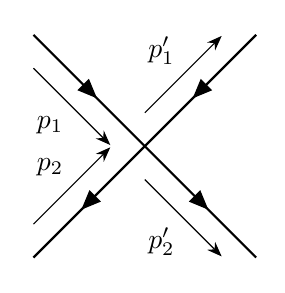
\begin{tikzpicture}
\begin{feynman}[large, baseline = (a)]
\vertex (i1) ;
\vertex [below right=of i1] (a);
\vertex [below left=of a] (i2);
\vertex [below right=of a] (f2);
\vertex [above right=of a] (f1);
\diagram* {
(i1) -- [fermion, momentum' = \(p_1\)] (a) -- [fermion, rmomentum' = \(p_2\)] (i2),
(f1) -- [fermion, rmomentum' = \(p_1'\)] (a) -- [fermion, momentum' = \(p_2'\)] (f2)
};
\end{feynman}
\end{tikzpicture}
\end{equation*}
Using the above Feynman rules,
\[ A = i (2 \pi)^4 \delta^4(p_1 + p_2 - p_1' - p_2') \left[ \frac{(- i g)^2}{(p_1 - p_1')^2 - m^2 + i \epsilon} + \frac{(- i g)^2}{(p_1 + p_2)^2 - m^2 + i \epsilon}  + (- 4 \lambda) \right] \]

\subsection*{(c)}

In the center of mass frame, $p_1 = (E, \vec{p})$ and $p_2 = (E, -\vec{p})$. Also, $p_1' = (E, \vec{p}')$ and $p_2' = (E, -\vec{p}')$. Then, $(p_1 + p_2)^2 = 4 E^2$ and $(p_1 - p_1')^2 = - (\Delta \vec{p})^{\,2}$. Therefore, in this frame, the scattering amplitude becomes,
\[ A = i (2 \pi)^4 \delta^4(p_1 + p_2 - p_1' - p_2') \left[ \frac{(- i g)^2}{4 E^2 - m^2 + i \epsilon} + \frac{(- i g)^2}{- (\Delta \vec{p})^{\,2} - m^2 + i \epsilon}  + (- 4 \lambda) \right] \]
In the limit $E^2 = \vec{p}^{\,2} + M^2 \to \infty$ if we also take $(\Delta \vec{p})^{\,2} \to \infty$, the scattering amplitude becomes,
\[A = (- 4i \lambda) (2 \pi)^4 \delta^4(p_1 + p_2 - p_1' - p_2')\]
Because they are scalars, each field has dimension $1$. Therefore, $g$ has dimension $1$ such that $g \dpsi \psi \meson$ has dimension $4$ to cancel $\dfourx$ which has dimension $-4$. Furthermore, $\lambda$ must be dimensionless such that $\lambda (\dpsi \psi)^2$ has dimension $4$ to cancel $\dfourx$ with dimension $-4$. Thus, the term proportional to $g$ is relevant and the term proportional to $\lambda$ is marginal. Therefore, in the high energy limit, the $g$ term is dominated by higher order terms. 
\section*{Problem 4.}
Consider the interaction Lagrangian,
\[ \lagrange_\ipic = -g \dpsi \psi \phi  - g'(\psi^2 + (\dpsi)^2) \phi \] 
\subsection*{(a)}
Here, there is a combinatorial factor of $2$ which appears in the $g'$ terms due to swapping the order of contraction of $\psi \psi$ or $\dpsi \dpsi$. This follows from the same argument used in part 3 (a). The possible interaction vertices are, 
	\begin{equation*}
	\feynmandiagram[horizontal = b to a, small, inline = (a)] {
	i1 -- [fermion] a -- [fermion] f1,
	a -- [scalar] b
	}; = - i g
	\hspace{2cm}
	\feynmandiagram[horizontal = b to a, small, inline = (a)] {
	i1 -- [anti fermion] a -- [fermion] f1,
	a -- [scalar] b
	}; = - 2 i g'
	\hspace{2cm}
	\feynmandiagram[horizontal = b to a, small, inline = (a)] {
	i1 -- [fermion] a -- [anti fermion] f1,
	a -- [scalar] b
	}; = - 2 i g'
	\end{equation*}
	\begin{itemize}
	\item Each internal meson line gives a factor of $\frac{i}{p^2 - m^2 + i \epsilon}$
	\item Each internal nucleon line gives a factor of $\frac{i}{p^2 - M^2 + i \epsilon}$
	\item Each $g$-vertex gives a factor of $(-ig) (2\pi)^4 \delta(\sum p)$
	\item Each $\psi\psi\phi$-vertex gives a factor of
	$(-2ig') (2\pi)^4 \delta(\sum p) $
	\item Each $\psi^\dag\psi^\dag\phi$-vertex gives a factor of
	$(-2ig')(2\pi)^4 \delta(\sum p)$
	\item Integrate over all undetermined momenta with measure $\int \frac{\d{^4p}}{(2\pi)^4}$
	\end{itemize}

\subsection*{(b)}

\begin{enumerate}
\item[i.] For $g' = 0$, the Lagrangian exhibits the $U(1)$ symmetry given by $\psi \mapsto e^{i \alpha} \psi$. Therefore, there is a conserved charge which does not allow the number of nucleons minus antinucleons to change. Since a stat e initially with two $\phi$ mesons has zero charge, the final state must also have zero charge. The only two particle states with zero charge are, $\phi \phi \to \phi \phi$ and $\phi \phi \mapsto \psi \bar{\psi}$. These processes are given, at lowest order, by the Feynman diagrams,
\begin{figure}
\centering
\begin{minipage}{.5\textwidth}
  \centering
  
\begin{tikzpicture}
\begin{feynman}
\vertex (i1) ;
\vertex [below right=of i1] (s1);
\vertex [right=of s1] (s2);
\vertex [below=of s2] (s3);
\vertex [left=of s3] (s4);
\vertex [below left=of s4] (i2);
\vertex [below right=of s3] (f2);
\vertex [above right=of s2] (f1);
\diagram* {
(i1) -- [scalar] (s1),
(i2) -- [scalar] (s4),
(f1) -- [scalar] (s2),
(f2) -- [scalar] (s3),
(s1) -- [fermion] (s2) -- [fermion] (s3) -- [fermion] (s4) -- [fermion] (s1),
};
\end{feynman}
\end{tikzpicture}
\caption{$\phi \phi \to \phi \phi$}
\end{minipage}%
\begin{minipage}{.5\textwidth}
  \centering
  
\begin{tikzpicture}
\begin{feynman}
\vertex (i1) ;
\vertex [below right=of i1] (s1);
\vertex [below=of s1] (s2);
\vertex [below left=of s2] (i2);
\vertex [below right=of s2] (f2);
\vertex [above right=of s1] (f1);
\diagram* {
(i1) -- [scalar] (s1),
(i2) -- [scalar] (s2),
(f1) -- [fermion] (s1) -- [fermion] (s2) -- [fermion] (f2)
};
\end{feynman}
\end{tikzpicture}
\caption{$\phi \phi \to \psi \bar{\psi}$}
\end{minipage}
\end{figure}
It it clear that other decay products are impossible due to the form of the vertex rules.

\item[ii.]

First consider the $\phi \phi \to \phi \phi$ process. There are three such diagrams at fourth order. Writing the momentum in the Feynman diagram,
\begin{figure}
\centering
\begin{minipage}{.33\textwidth}
\begin{center}
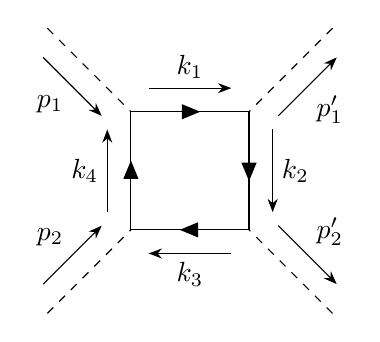
\begin{tikzpicture}
\begin{feynman}
\vertex (i1) ;
\vertex [below right=of i1] (s1);
\vertex [right=of s1] (s2);
\vertex [below=of s2] (s3);
\vertex [left=of s3] (s4);
\vertex [below left=of s4] (i2);
\vertex [below right=of s3] (f2);
\vertex [above right=of s2] (f1);
\diagram* {
(i1) -- [scalar, momentum' = \(p_1\)] (s1),
(i2) -- [scalar, momentum = \(p_2\)] (s4),
(f1) -- [scalar, rmomentum = \(p_1'\)] (s2),
(f2) -- [scalar, rmomentum' = \(p_2'\)] (s3),
(s1) -- [fermion, momentum = \(k_1\)] (s2) -- [fermion, momentum = \(k_2\)] (s3) -- [fermion, momentum = \(k_3\)] (s4) -- [fermion, momentum = \(k_4\)] (s1),
};
\end{feynman}
\end{tikzpicture}
\end{center}
\end{minipage}%
\begin{minipage}{.33\textwidth}
\begin{center}
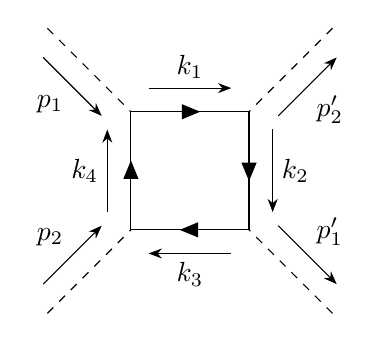
\begin{tikzpicture}
\begin{feynman}
\vertex (i1) ;
\vertex [below right=of i1] (s1);
\vertex [right=of s1] (s2);
\vertex [below=of s2] (s3);
\vertex [left=of s3] (s4);
\vertex [below left=of s4] (i2);
\vertex [below right=of s3] (f2);
\vertex [above right=of s2] (f1);
\diagram* {
(i1) -- [scalar, momentum' = \(p_1\)] (s1),
(i2) -- [scalar, momentum = \(p_2\)] (s4),
(f1) -- [scalar, rmomentum = \(p_2'\)] (s2),
(f2) -- [scalar, rmomentum' = \(p_1'\)] (s3),
(s1) -- [fermion, momentum = \(k_1\)] (s2) -- [fermion, momentum = \(k_2\)] (s3) -- [fermion, momentum = \(k_3\)] (s4) -- [fermion, momentum = \(k_4\)] (s1),
};
\end{feynman}
\end{tikzpicture}
\end{center}
\end{minipage}%
\begin{minipage}{.33\textwidth}
\begin{center}
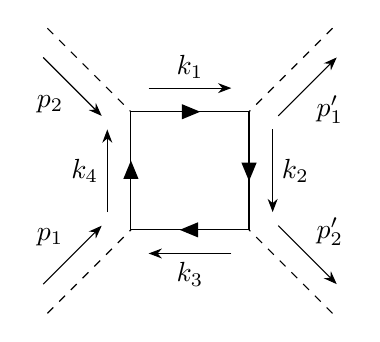
\begin{tikzpicture}
\begin{feynman}
\vertex (i1) ;
\vertex [below right=of i1] (s1);
\vertex [right=of s1] (s2);
\vertex [below=of s2] (s3);
\vertex [left=of s3] (s4);
\vertex [below left=of s4] (i2);
\vertex [below right=of s3] (f2);
\vertex [above right=of s2] (f1);
\diagram* {
(i1) -- [scalar, momentum' = \(p_2\)] (s1),
(i2) -- [scalar, momentum = \(p_1\)] (s4),
(f1) -- [scalar, rmomentum = \(p_1'\)] (s2),
(f2) -- [scalar, rmomentum' = \(p_2'\)] (s3),
(s1) -- [fermion, momentum = \(k_1\)] (s2) -- [fermion, momentum = \(k_2\)] (s3) -- [fermion, momentum = \(k_3\)] (s4) -- [fermion, momentum = \(k_4\)] (s1),
};
\end{feynman}
\end{tikzpicture}
\end{center}
\end{minipage}
\end{figure}

In the first diagram, $p_1 + k_4 = k_1$ and $p_2 + k_3 = k_4$ and $p_1' + k_2 = k_1$ and $p_2' + k_3 = k_2$. Thus, $k_2 = k_1 - p_1'$ and $k_3 = k_1  - p_1' - p_2'$ and $k_4 = k_1  - p_1$ so we have one unconstraned momentum. Using the Feynman rules,
\begin{align*}
A_1 = & (-ig)^4 (2 \pi)^4 \delta^4(p_1 + p_2 - p_1' - p_2')
\\
& \cdot \int \frac{\mathrm{d}^4 k_1}{(2 \pi)^4} \left[ \frac{i}{k_1^2 - M^2 + i \epsilon} \frac{i}{(k_1 - p_1')^2 - M^2 + i \epsilon}  \frac{i}{(k_1 - p_1' - p_2')^2 - M^2 + i \epsilon} \frac{i}{(k_1 - p_1)^2 - M^2 + i \epsilon}  \right] 
\end{align*}
Similarly, swapping $p_1'$ and $p_2'$ to get the second diagram,
\begin{align*}
A_2 = & (-ig)^4 (2 \pi)^4 \delta^4(p_1 + p_2 - p_1' - p_2')
\\
& \cdot \int \frac{\mathrm{d}^4 k_1}{(2 \pi)^4} \left[ \frac{i}{k_1^2 - M^2 + i \epsilon} \frac{i}{(k_1 - p_2')^2 - M^2 + i \epsilon}  \frac{i}{(k_1 - p_2' - p_1')^2 - M^2 + i \epsilon} \frac{i}{(k_1 - p_1)^2 - M^2 + i \epsilon}  \right] 
\end{align*}
Finally, swapping $p_1$ and $p_2$ for the third diagram,
\begin{align*}
A_1 = & (-ig)^4 (2 \pi)^4 \delta^4(p_1 + p_2 - p_1' - p_2')
\\
& \cdot \int \frac{\mathrm{d}^4 k_1}{(2 \pi)^4} \left[ \frac{i}{k_1^2 - M^2 + i \epsilon} \frac{i}{(k_1 - p_1')^2 - M^2 + i \epsilon}  \frac{i}{(k_1 - p_1' - p_2')^2 - M^2 + i \epsilon} \frac{i}{(k_1 - p_2)^2 - M^2 + i \epsilon}  \right] 
\end{align*}
Likewise there are another three diagrams which come from reversing the arrows on the central loop,
\begin{figure}
\centering
\begin{minipage}{.33\textwidth}
\begin{center}
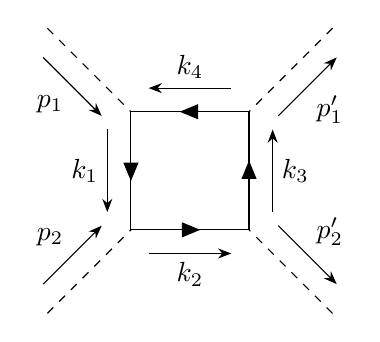
\begin{tikzpicture}
\begin{feynman}
\vertex (i1) ;
\vertex [below right=of i1] (s1);
\vertex [right=of s1] (s2);
\vertex [below=of s2] (s3);
\vertex [left=of s3] (s4);
\vertex [below left=of s4] (i2);
\vertex [below right=of s3] (f2);
\vertex [above right=of s2] (f1);
\diagram* {
(i1) -- [scalar, momentum' = \(p_1\)] (s1),
(i2) -- [scalar, momentum = \(p_2\)] (s4),
(f1) -- [scalar, rmomentum = \(p_1'\)] (s2),
(f2) -- [scalar, rmomentum' = \(p_2'\)] (s3),
(s1) -- [fermion, momentum' = \(k_1\)] (s4) -- [fermion, momentum' = \(k_2\)] (s3) -- [fermion, momentum' = \(k_3\)] (s2) -- [fermion, momentum' = \(k_4\)] (s1),
};
\end{feynman}
\end{tikzpicture}
\end{center}
\end{minipage}%
\begin{minipage}{.33\textwidth}
\begin{center}
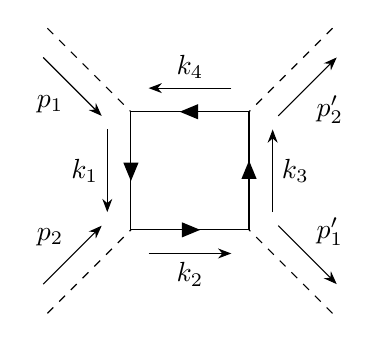
\begin{tikzpicture}
\begin{feynman}
\vertex (i1) ;
\vertex [below right=of i1] (s1);
\vertex [right=of s1] (s2);
\vertex [below=of s2] (s3);
\vertex [left=of s3] (s4);
\vertex [below left=of s4] (i2);
\vertex [below right=of s3] (f2);
\vertex [above right=of s2] (f1);
\diagram* {
(i1) -- [scalar, momentum' = \(p_1\)] (s1),
(i2) -- [scalar, momentum = \(p_2\)] (s4),
(f1) -- [scalar, rmomentum = \(p_2'\)] (s2),
(f2) -- [scalar, rmomentum' = \(p_1'\)] (s3),
(s1) -- [fermion, momentum' = \(k_1\)] (s4) -- [fermion, momentum' = \(k_2\)] (s3) -- [fermion, momentum' = \(k_3\)] (s2) -- [fermion, momentum' = \(k_4\)] (s1),
};
\end{feynman}
\end{tikzpicture}
\end{center}
\end{minipage}%
\begin{minipage}{.33\textwidth}
\begin{center}
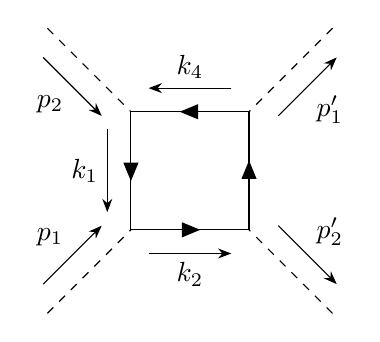
\begin{tikzpicture}
\begin{feynman}
\vertex (i1) ;
\vertex [below right=of i1] (s1);
\vertex [right=of s1] (s2);
\vertex [below=of s2] (s3);
\vertex [left=of s3] (s4);
\vertex [below left=of s4] (i2);
\vertex [below right=of s3] (f2);
\vertex [above right=of s2] (f1);
\diagram* {
(i1) -- [scalar, momentum' = \(p_2\)] (s1),
(i2) -- [scalar, momentum = \(p_1\)] (s4),
(f1) -- [scalar, rmomentum = \(p_1'\)] (s2),
(f2) -- [scalar, rmomentum' = \(p_2'\)] (s3),
(s1) -- [fermion, momentum' = \(k_1\)] (s4) -- [fermion, momentum' = \(k_2\)] (s3) -- [fermion,  ' = \(k_3\)] (s2) -- [fermion, momentum' = \(k_4\)] (s1),
};
\end{feynman}
\end{tikzpicture}
\end{center}
\end{minipage}
\end{figure}
Because the integral over $k$ runs over all values, these diagrams give an identical contribution. Finally, combing these diagrams, the total amplitude for the process is, $A = 2(A_1 + A_2 + A_3)$.
\bigskip \\
Next, consider the $\phi \phi \to \psi \bar{\psi}$ process. Again, there are two diagrams which contribute at (leading) second order. Writing the diagrams with momenta, 

\begin{figure}
\centering
\begin{minipage}{.5\textwidth}
\begin{center}
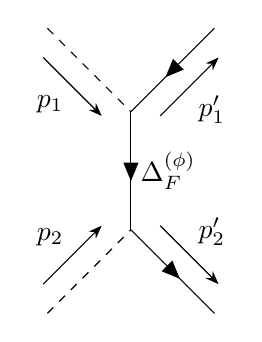
\begin{tikzpicture}
\begin{feynman}
\vertex (i1) ;
\vertex [below right=of i1] (s1);
\vertex [below=of s1] (s2);
\vertex [below left=of s2] (i2);
\vertex [below right=of s2] (f2);
\vertex [above right=of s1] (f1);
\diagram* {
(i1) -- [scalar, momentum' = \(p_1\)] (s1),
(i2) -- [scalar, momentum = \(p_2\)] (s2),
(f1) -- [fermion, rmomentum = \(p_1'\)] (s1) -- [fermion, edge label = \(\Delta^{(\phi)}_F\)] (s2) -- [fermion, momentum = \(p_2'\)] (f2)
};
\end{feynman}
\end{tikzpicture}
\end{center}
\end{minipage}%
\begin{minipage}{.5\textwidth}
\begin{center}
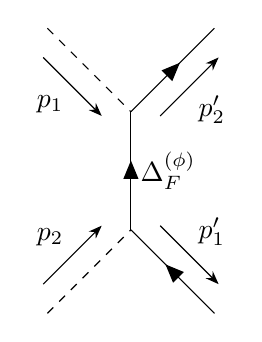
\begin{tikzpicture}
\begin{feynman}
\vertex (i1) ;
\vertex [below right=of i1] (s1);
\vertex [below=of s1] (s2);
\vertex [below left=of s2] (i2);
\vertex [below right=of s2] (f2);
\vertex [above right=of s1] (f1);
\diagram* {
(i1) -- [scalar, momentum' = \(p_1\)] (s1),
(i2) -- [scalar, momentum = \(p_2\)] (s2),
(f2) -- [fermion, rmomentum' = \(p_1'\)] (s2) -- [fermion, edge label' = \(\Delta^{(\phi)}_F\)] (s1) -- [fermion, momentum' = \(p_2'\)] (f1)
};
\end{feynman}
\end{tikzpicture}
\end{center}
\end{minipage}
\end{figure}

All the momenta are constrained so we need not do any annyoing loop integrals. Therefore, the scattering amplitude can be found easily from the Feynman rules,
\[ A = (-ig)^2 (2 \pi)^4 \delta(p_1 + p_2 - p_1' - p_2') \left[ \frac{i}{(p_1 - p_1')^2 - M^2 + i \epsilon} + \frac{i}{(p_1 - p_2')^2 - m^2 + i \epsilon} \right] \]

\item[iii.]

If $g' \neq 0$ then the new term in the Lagrangian alows for the production of $\psi \psi$ or $\dpsi \bar{\psi}$ at a vertex. Therefore, since we already have $\phi \phi \to \phi \phi$ and $\phi \phi \to \psi \bar{\psi}$ now we add the new possibilities $\phi \phi \to \psi \psi$ and $\phi \phi \to \bar{\psi} \bar{\psi}$. Therefore, a $\phi \phi$ collision can produce any pair of particles under the new Lagrangian.

\item[iv.] 
As seen above, the nontrivial $\phi \phi \to \phi \phi$ process only enters at order $g^4$ or equivalent \footnote{Using the new interaction terms we can make a nucleon square loop with $g'$ vertices instead or half-and-half $g$ and $g'$ vertices. Therefore, it would be more accurate to say the $\phi \phi \to \phi \phi$ process enters at order $g^4$ or $(gg')^2$ or $g'^4$}. However, the process $\phi \phi \to \psi \bar{\psi}$ enters at order $g^2$ or $g'^2$ by reversing the interior line. The new processes enter at order $g g'$ with the diagrams, 

\begin{figure}
\centering
\begin{minipage}{.5\textwidth}
\begin{center}
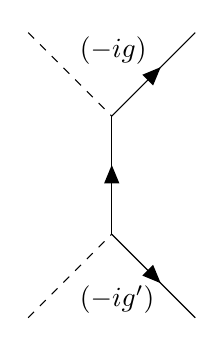
\begin{tikzpicture}
\begin{feynman}
\vertex (i1) ;
\vertex [below right=of i1] (s1);
\vertex [below=of s1] (s2);
\vertex [below left=of s2] (i2);
\vertex [below right=of s2] (f2);
\vertex [above right=of s1] (f1);
\diagram* {
(i1) -- [scalar, edge label = \((-ig)\)] (s1),
(i2) -- [scalar, edge label' = \((-ig')\)] (s2),
(s2) -- [fermion] (s1) -- [fermion] (f1),
(s2) -- [fermion] (f2)
};
\end{feynman}
\end{tikzpicture}
\end{center}
\end{minipage}%
\begin{minipage}{.5\textwidth}
\begin{center}
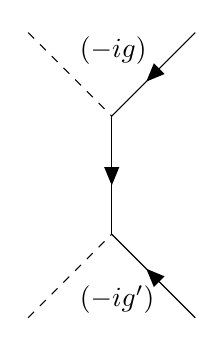
\begin{tikzpicture}
\begin{feynman}
\vertex (i1) ;
\vertex [below right=of i1] (s1);
\vertex [below=of s1] (s2);
\vertex [below left=of s2] (i2);
\vertex [below right=of s2] (f2);
\vertex [above right=of s1] (f1);
\diagram* {
(i1) -- [scalar, edge label = \((-ig)\)] (s1),
(i2) -- [scalar, edge label' = \((-ig')\)] (s2),
(f1) -- [fermion] (s1) -- [fermion] (s2),
(f2) -- [fermion] (s2)
};
\end{feynman}
\end{tikzpicture}
\end{center}
\end{minipage}
\end{figure}

\end{enumerate}

\subsection*{(c)}
Let $g' = \frac{g}{2}$ such that $\lagrange_{\ipic} = - \frac{g}{2} \left( \psi + \dpsi \right)^2 \phi$. Define the `meson' fields,
\[\sigma_{+} = \tfrac{1}{\sqrt{2}} \left( \psi + \dpsi \right) \quad \text{and} \quad \sigma_{-} = \tfrac{i}{\sqrt{2}} \left( \dpsi - \psi \right)\]
\begin{enumerate}
\item[i.] 
We can write the nucleon fields in terms of our new meson fields as,
\[ \psi = \tfrac{1}{\sqrt{2}} \left( \sigma_{+} + i \sigma_{-} \right) \quad \text{and} \quad \dpsi = \tfrac{1}{\sqrt{2}} \left( \sigma_{+} - i \sigma_{-} \right) \]
Thus, the full Lagrangian can be written as,
\begin{align*}
\lagrange = \lagrange_0 + \lagrange_{\ipic} & = \tfrac{1}{2} (\partial \phi)^2 - \tfrac{1}{2} m^2 \phi^2 + \partial_\mu \dpsi \partial^\mu \psi - M^2 \dpsi \psi - \frac{g}{2} \left( \psi + \dpsi \right)^2 \phi 
\\
& = \tfrac{1}{2} (\partial \phi)^2 - \tfrac{1}{2} m^2 \phi^2 + \tfrac{1}{2}\partial_\mu (\sigma_{+} - i \sigma_{-}) \partial^\mu (\sigma_{+} + i \sigma_{-}) - \tfrac{1}{2} M^2 (\sigma_{+} - i \sigma_{-})(\sigma_{+} + i \sigma_{-}) - g \sigma_{+}^2 \phi 
\\
& = \tfrac{1}{2} (\partial \phi)^2 - \tfrac{1}{2} m^2 \phi^2 + \tfrac{1}{2}(\partial \sigma_+)^2 + \tfrac{1}{2} (\partial \sigma_{-})^2 - \tfrac{1}{2} M^2 (\sigma_{+}^2 + \sigma_{-}^2) - g \sigma_{+}^2 \phi 
\end{align*}
\item[ii.]
The interacting Lagrangian has no terms including $\sigma_-$. Therfore, $\sigma_-$ cannot be contracted at any vertex. For $\sigma_+$ mesons we use a solid line to denote the particle. There is only a single vertex type of vetex:
	\begin{equation*}
	\feynmandiagram [small, baseline=(d.base), horizontal=d to b] {
	a -- b -- c,
	b -- [scalar] d
	};
	= - 2i g
	\end{equation*}
	\renewcommand{\theenumiii}{(\roman{enumiii})}
	which enters with a factor of $2$ because there is freedom to contract $\sigma_+^2$ in two different ways.
	\begin{enumerate}
	\item Each internal $\phi$ line gives a factor of $\frac{i}{p^2 - m^2 + i \epsilon}$
	\item Each internal $\sigma_+$ line gives a factor of $\frac{i}{p^2 - M^2 + i \epsilon}$
	\item Each vertex gives a factor of $(-2ig) (2\pi)^4 \delta(p_\text{tot}) $, where
	$p_\text{tot}$ is the total momentum incoming to the vertex
	\item Integrate over all undetermined momenta with measure $\int \frac{\d{^4p}}{(2\pi)^4}$
	\end{enumerate}

\item[iii.]
The possible 2-particle processes from a $\phi \phi$ collision are, $\phi \phi \to \phi \phi$ and $\phi \phi \to \sigma_{+} \sigma_{+}$. There is no interaction term with a $\sigma_{-}$ meson field so we cannot have an outgoing $\sigma_{-}$. Furthermore, the process $\phi \phi \to \sigma_{+} \phi$ is not allowed because the Lagrangian is invariant under $\sigma_{+} \mapsto - \sigma_{+}$. Therefore, the operator taking $\sigma_{+} \mapsto - \sigma_{+}$ commutes with time-evolution. Since the initial state (with no $\sigma_{+}$) is even under this transformation, the final state must also be even under $\sigma_{+} \mapsto - \sigma_{+}$ so it must have an even number of $\sigma_{+}$ mesons. These processes are given, at leading order, by the diagrams,
\begin{figure}
\centering
\begin{minipage}{.5\textwidth}
  \centering
  
\begin{tikzpicture}
\begin{feynman}
\vertex (i1) ;
\vertex [below right=of i1] (s1);
\vertex [right=of s1] (s2);
\vertex [below=of s2] (s3);
\vertex [left=of s3] (s4);
\vertex [below left=of s4] (i2);
\vertex [below right=of s3] (f2);
\vertex [above right=of s2] (f1);
\diagram* {
(i1) -- [scalar] (s1),
(i2) -- [scalar] (s4),
(f1) -- [scalar] (s2),
(f2) -- [scalar] (s3),
(s1) -- (s2) -- (s3) -- (s4) -- (s1),
};
\end{feynman}
\end{tikzpicture}
\caption{$\phi \phi \to \phi \phi$}
\end{minipage}%
\begin{minipage}{.5\textwidth}
  \centering
  
\begin{tikzpicture}
\begin{feynman}
\vertex (i1) ;
\vertex [below right=of i1] (s1);
\vertex [below=of s1] (s2);
\vertex [below left=of s2] (i2);
\vertex [below right=of s2] (f2);
\vertex [above right=of s1] (f1);
\diagram* {
(i1) -- [scalar] (s1),
(i2) -- [scalar] (s2),
(f1) -- (s1) -- (s2) -- (f2)
};
\end{feynman}
\end{tikzpicture}
\caption{$\phi \phi \to \sigma_{+} \sigma_{+}$}
\end{minipage}
\end{figure}
where solid lines represent $\sigma_{+}$ mesons.
\item[iv.]
First consider the $\phi \phi \to \phi \phi$ process. There are three such diagrams at four order. Writing the momentum in the Feynman diagram,
\begin{figure}
\centering
\begin{minipage}{.33\textwidth}
\begin{center}
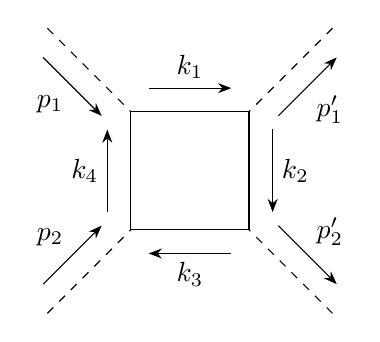
\begin{tikzpicture}
\begin{feynman}
\vertex (i1) ;
\vertex [below right=of i1] (s1);
\vertex [right=of s1] (s2);
\vertex [below=of s2] (s3);
\vertex [left=of s3] (s4);
\vertex [below left=of s4] (i2);
\vertex [below right=of s3] (f2);
\vertex [above right=of s2] (f1);
\diagram* {
(i1) -- [scalar, momentum' = \(p_1\)] (s1),
(i2) -- [scalar, momentum = \(p_2\)] (s4),
(f1) -- [scalar, rmomentum = \(p_1'\)] (s2),
(f2) -- [scalar, rmomentum' = \(p_2'\)] (s3),
(s1) -- [momentum = \(k_1\)] (s2) -- [momentum = \(k_2\)] (s3) -- [momentum = \(k_3\)] (s4) -- [momentum = \(k_4\)] (s1),
};
\end{feynman}
\end{tikzpicture}
\end{center}
\end{minipage}%
\begin{minipage}{.33\textwidth}
\begin{center}
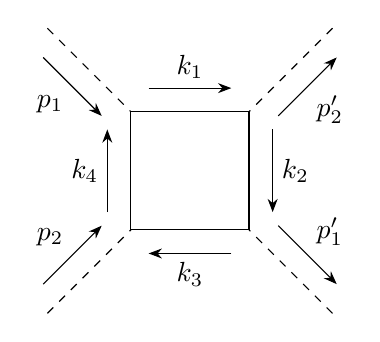
\begin{tikzpicture}
\begin{feynman}
\vertex (i1) ;
\vertex [below right=of i1] (s1);
\vertex [right=of s1] (s2);
\vertex [below=of s2] (s3);
\vertex [left=of s3] (s4);
\vertex [below left=of s4] (i2);
\vertex [below right=of s3] (f2);
\vertex [above right=of s2] (f1);
\diagram* {
(i1) -- [scalar, momentum' = \(p_1\)] (s1),
(i2) -- [scalar, momentum = \(p_2\)] (s4),
(f1) -- [scalar, rmomentum = \(p_2'\)] (s2),
(f2) -- [scalar, rmomentum' = \(p_1'\)] (s3),
(s1) -- [momentum = \(k_1\)] (s2) -- [momentum = \(k_2\)] (s3) -- [momentum = \(k_3\)] (s4) -- [momentum = \(k_4\)] (s1),
};
\end{feynman}
\end{tikzpicture}
\end{center}
\end{minipage}%
\begin{minipage}{.33\textwidth}
\begin{center}
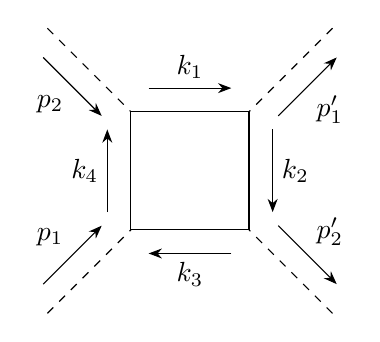
\begin{tikzpicture}
\begin{feynman}
\vertex (i1) ;
\vertex [below right=of i1] (s1);
\vertex [right=of s1] (s2);
\vertex [below=of s2] (s3);
\vertex [left=of s3] (s4);
\vertex [below left=of s4] (i2);
\vertex [below right=of s3] (f2);
\vertex [above right=of s2] (f1);
\diagram* {
(i1) -- [scalar, momentum' = \(p_2\)] (s1),
(i2) -- [scalar, momentum = \(p_1\)] (s4),
(f1) -- [scalar, rmomentum = \(p_1'\)] (s2),
(f2) -- [scalar, rmomentum' = \(p_2'\)] (s3),
(s1) -- [momentum = \(k_1\)] (s2) -- [momentum = \(k_2\)] (s3) -- [momentum = \(k_3\)] (s4) -- [momentum = \(k_4\)] (s1),
};
\end{feynman}
\end{tikzpicture}
\end{center}
\end{minipage}
\end{figure}

In the first diagram, $p_1 + k_4 = k_1$ and $p_2 + k_3 = k_4$ and $p_1' + k_2 = k_1$ and $p_2' + k_3 = k_2$. Thus, $k_2 = k_1 - p_1'$ and $k_3 = k_1  - p_1' - p_2'$ and $k_4 = k_1  - p_1$ so we have one unconstraned momentum. Using the Feynman rules,
\begin{align*}
A_1 = & (-2ig)^4 (2 \pi)^4 \delta^4(p_1 + p_2 - p_1' - p_2')
\\
& \cdot \int \frac{\mathrm{d}^4 k_1}{(2 \pi)^4} \left[ \frac{i}{k_1^2 - M^2 + i \epsilon} \frac{i}{(k_1 - p_1')^2 - M^2 + i \epsilon}  \frac{i}{(k_1 - p_1' - p_2')^2 - M^2 + i \epsilon} \frac{i}{(k_1 - p_1)^2 - M^2 + i \epsilon}  \right] 
\end{align*}
Similarly, for the second diagram, we need only swap $p_1'$ and $p_2'$,
\begin{align*}
A_2 = & (-2ig)^4 (2 \pi)^4 \delta^4(p_1 + p_2 - p_1' - p_2')
\\
& \cdot \int \frac{\mathrm{d}^4 k_1}{(2 \pi)^4} \left[ \frac{i}{k_1^2 - M^2 + i \epsilon} \frac{i}{(k_1 - p_2')^2 - M^2 + i \epsilon}  \frac{i}{(k_1 - p_2' - p_1')^2 - M^2 + i \epsilon} \frac{i}{(k_1 - p_1)^2 - M^2 + i \epsilon}  \right] 
\end{align*}
Finally, the third diagram comes from swapping $p_1$ and $p_2$,
\begin{align*}
A_3 = & (-2ig)^4 (2 \pi)^4 \delta^4(p_1 + p_2 - p_1' - p_2')
\\
& \cdot \int \frac{\mathrm{d}^4 k_1}{(2 \pi)^4} \left[ \frac{i}{k_1^2 - M^2 + i \epsilon} \frac{i}{(k_1 - p_1')^2 - M^2 + i \epsilon}  \frac{i}{(k_1 - p_1' - p_2')^2 - M^2 + i \epsilon} \frac{i}{(k_1 - p_2)^2 - M^2 + i \epsilon}  \right] 
\end{align*}
At last, $A = A_1 + A_2 + A_3$.
\bigskip \\
Next, consider the $\phi \phi \to \psi \bar{\psi}$ process. Again, there are two diagrams which contribute at (leading) second order. Writing the diagrams with momenta, 

\begin{figure}
\centering
\begin{minipage}{.5\textwidth}
\begin{center}
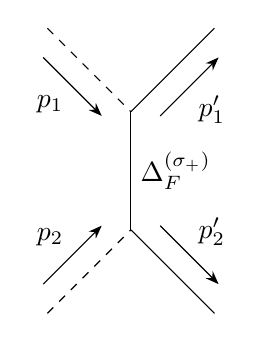
\begin{tikzpicture}
\begin{feynman}
\vertex (i1) ;
\vertex [below right=of i1] (s1);
\vertex [below=of s1] (s2);
\vertex [below left=of s2] (i2);
\vertex [below right=of s2] (f2);
\vertex [above right=of s1] (f1);
\diagram* {
(i1) -- [scalar, momentum' = \(p_1\)] (s1),
(i2) -- [scalar, momentum = \(p_2\)] (s2),
(f1) -- [rmomentum = \(p_1'\)] (s1) -- [edge label = \(\Delta^{(\sigma_{+})}_F\)] (s2) -- [momentum = \(p_2'\)] (f2)
};
\end{feynman}
\end{tikzpicture}
\end{center}
\end{minipage}%
\begin{minipage}{.5\textwidth}
\begin{center}
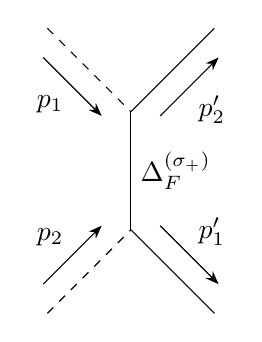
\begin{tikzpicture}
\begin{feynman}
\vertex (i1) ;
\vertex [below right=of i1] (s1);
\vertex [below=of s1] (s2);
\vertex [below left=of s2] (i2);
\vertex [below right=of s2] (f2);
\vertex [above right=of s1] (f1);
\diagram* {
(i1) -- [scalar, momentum' = \(p_1\)] (s1),
(i2) -- [scalar, momentum = \(p_2\)] (s2),
(f2) -- [rmomentum' = \(p_1'\)] (s2) -- [edge label' = \(\Delta^{(\sigma_{+})}_F\)] (s1) -- [momentum' = \(p_2'\)] (f1)
};
\end{feynman}
\end{tikzpicture}
\end{center}
\end{minipage}
\end{figure}

All the momenta are constrained so we need not do any annyoing loop integrals. Therefore, the scattering amplitude can be found easily from the Feynman rules,
\[ A = (-2ig)^2 (2 \pi)^4 \delta^4(p_1 + p_2 - p_1' - p_2') \left[ \frac{i}{(p_1 - p_1')^2 - M^2 + i \epsilon} + \frac{i}{(p_1 - p_2')^2 - m^2 + i \epsilon} \right] \]

\end{enumerate}

\end{document}

